 % The main file for CAMP reports
 % Don't put any content in here. 
 % Don't even include content files by using \input or \inlcude. 
 % Put your content to TEXT.TEX or include it there using \input.
 % Uses:
 %		SETTINGS.TEX	contains the settings for this document
 %		COMMANDS.TEX	contains commands which can be used while writing
 %		INFO.TEX			contains the author, title and so on for the cover
 %		COVER.TEX			formats the front cover of the document
 %		ABSTRACT.TEX	contains the abstract to be included (if needed)
 %		TEXT.TEX			contains the actual content of the document
 %		BIB.BIB				containt the BibTeX entries for the document


%% Draft document mode
%% Final document
\documentclass[11pt,a4paper,bibtotoc,idxtotoc,headsepline,footsepline,footexclude,BCOR12mm,DIV13]{scrbook}

%\documentclass[11pt,a4paper,bibtotoc,idxtotoc,headsepline,footsepline,footexclude,BCOR20mm,DIV10]{scrbook}

% KOMA-Optionen:
%  bibtotoc: include bibliography in table of contents
%  idxtotoc: include index in table of contents
%  headsepline: use horizontalline under heading
%  BCOR: binding correcion (Bindungskorrektur) (e.g.: BCOR5mm)
%  DIV: Number of sheet sections (used for layout) (e.g.: DIV12) 



% include title and author information for the cover
% Set here the title, authors and other stuff to be used for the cover
% This file is used by MAIN.TEX

% set title, authors and stuff for the cover
\def\doctype{Masterarbeit in Informatik}
\def\title{Runtime Protection against Advanced Code Reuse Attacks by Static Instrumentation of Binaries}
\def\titleGer{Laufzeitschutz gegen fortgeschrittene Code Wiederverwendungs-Angriffe durch statische Instrumentierung von Bin{\"a}rdateien}
\def\author{Matthias Konstantin Fischer}
\def\date{November 7th, 2016}

% text to appear in the footer
\def\footertext{}

% include settings
% Included by MAIN.TEX
% Defines the settings for the CAMP report document

\renewcommand{\sectfont}{\normalfont \bfseries}        % Schriftart der Kopfzeile

% manipulate footer
\usepackage{scrpage2}
\pagestyle{scrheadings}
\ifoot[\footertext]{\footertext} % \footertext set in INFO.TEX
%\setkomafont{pagehead}{\normalfont\rmfamily}
\setkomafont{pagenumber}{\normalfont\rmfamily}

%% allow sophisticated control structures
\usepackage{ifthen}

% use Palatino as default font
\usepackage{palatino}

% enable special PostScript fonts
\usepackage{pifont}

% make thumbnails
\usepackage{thumbpdf}

%to use the subfigures
\usepackage{subfigure}


\usepackage{colortbl}


%% show program code\ldots
%\usepackage{verbatim}
%\usepackage{program}

%% enable TUM symbols on title page
\usepackage{styles/tumlogo}


\usepackage{multirow}

%% use colors
\usepackage{color}

%% make fancy math
\usepackage{amsmath}
\usepackage{amsfonts}
\usepackage{amssymb}
\usepackage{textcomp}
\usepackage{yhmath} % f�r die adots 
%% mark text as preliminary
%\usepackage[draft,german,scrtime]{prelim2e}

%% create an index
\usepackage{makeidx}

% for the program environment
\usepackage{float}

%% load german babel package for german abstract
%\usepackage[german,american]{babel}
\usepackage[german,english, croatian]{babel}
\selectlanguage{english}
% use german characters as well
\usepackage[latin1, utf8]{inputenc}       % allow Latin1 characters

% use initals dropped caps - doesn't work with PDF
%\usepackage{dropping}


\usepackage{styles/shortoverview}
%----------------------------------------------------
%      Graphics and Hyperlinks
%----------------------------------------------------

%% check for pdfTeX
\ifx\pdftexversion\undefined
 %% use PostScript graphics
 \usepackage[dvips]{graphicx}
 \DeclareGraphicsExtensions{.eps,.epsi}
 \graphicspath{{figures/}{figures/review}} 
 %% allow rotations
 \usepackage{rotating}
 %% mark pages as draft copies
 %\usepackage[english,all,light]{draftcopy}
 %% use hypertex version of hyperref
 \usepackage[hypertex,hyperindex=false,colorlinks=false]{hyperref}
\else %% reduce output size \pdfcompresslevel=9
 %% declare pdfinfo
 %\pdfinfo { 
 %  /Title (my title) 
 %  /Creator (pdfLaTeX) 
 %  /Author (my name) 
 %  /Subject (my subject	) 
 %  /Keywords (my keywords)
 %}
 %% use pdf or jpg graphics
 \usepackage[pdftex]{graphicx}
 \DeclareGraphicsExtensions{.jpg,.JPG,.png,.pdf,.eps}
 \graphicspath{{figures/}} 
 
 %% Load float package, for enabling floating extensions
 \usepackage{float}
 
 %% allow rotations
 \usepackage{rotating}
 %% use pdftex version of hyperref
 \usepackage[pdftex,colorlinks=true,linkcolor=red,citecolor=red,%
 anchorcolor=red,urlcolor=red,bookmarks=true,%
 bookmarksopen=true,bookmarksopenlevel=0,plainpages=false%
 bookmarksnumbered=true,hyperindex=false,pdfstartview=%
 ]{hyperref}
%
%\usepackage[pdftex,colorlinks=false,linkcolor=red,citecolor=red,%
% anchorcolor=red,urlcolor=red,bookmarks=true,%
% bookmarksopen=true,bookmarksopenlevel=0,plainpages=false%
% bookmarksnumbered=true,hyperindex=false,pdfstartview=%
% ]{hyperref}
\fi




%% Fancy chapters
%\usepackage[Lenny]{fncychap}
%\usepackage[Glenn]{fncychap}
%\usepackage[Bjarne]{fncychap}

%\usepackage[avantgarde]{quotchap}

% set the bibliography style
%\bibliographystyle{styles/bauermaNum}
%\bibliographystyle{alpha}
\bibliographystyle{plain}

% include commands
% Commands to be used within the TUM report document
% Included by MAIN.TEX
% Please include your own cool commands here. 
% Be only sure to comment it sufficiently so others can use it.

%-------------------------------------------------------------
%                      Own Commands
%-------------------------------------------------------------


%-------------------------------------------------------------
% math stuff -------------------------------------------------

% nice R, N, C
\newcommand{\nat}{\mathbb{N}}
\newcommand{\real}{\mathbb{R}}
\newcommand{\compl}{\mathbb{C}}



% norm
\newcommand{\norm}[1]{\left\| #1 \right\|}

% un demi
\newcommand{\half}{\frac{1}{2}}

% parantheses
\newcommand{\parenth}[1]{ \left( #1 \right) }
\newcommand{\bracket}[1]{ \left[ #1 \right] }
\newcommand{\accolade}[1]{ \left\{ #1 \right\} }
%\newcommand{\angle}[1]{ \left\langle  #1 \right\rangle }

% partial derivative: %#1 function, #2 which variable
% simple / single line version
\newcommand{\pardevS}[2]{ \delta_{#1} f(#2) }
% fraction version
\newcommand{\pardevF}[2]{ \frac{\partial #1}{\partial #2} }

% render vectors: 3 and 4 dimensional
\newcommand{\veciii}[3]{\left[ \begin{array}[h]{c} #1 \\ #2 \\ #3	\end{array} \right]}
\newcommand{\veciv}[4]{\left[ \begin{array}[h]{c} #1 \\ #2 \\ #3 \\ #4	\end{array} \right]}

% render matrices: 3  dimensional (arguments in row first order)
\newcommand{\matiii}[9]{\left[ \begin{array}[h]{ccc} #1 & #2 & #3 \\ #4 & #5 & #6 \\ #7 & #8 & #9	\end{array} \right]}
%DOESN'T WORK,DON'T KNOW WHY \newcommand{\mativ}[16]{\left[ \begin{array}[h]{cccc} #1 & #2 & #3 & #4 \\ #5 & #6 & #7 & #8 \\ #9 & #10 & #11 & #12 \\ #13 & #14 & #15 & #16 \end{array} \right]}


%-------------------------------------------------------------
%-------------------------------------------------------------


%-------------------------------------------------------------
% some abreviations ------------------------------------------
\newcommand{\Reg}{$^{\textregistered}$}
\newcommand{\reg}{$^{\textregistered}$ }
\newcommand{\Tm}{\texttrademark}
\newcommand{\tm}{\texttrademark~}
\newcommand {\bsl} {$\backslash$}

%-------------------------------------------------------------
%-------------------------------------------------------------


%-------------------------------------------------------------
% formating --------------------------------------------------

% Theorem & Co environments and counters
\newtheorem{theorem}{Theorem}[chapter]
\newtheorem{lemma}[theorem]{Lemma}
\newtheorem{corollary}[theorem]{Corollary}
\newtheorem{remark}[theorem]{Remark}
\newtheorem{definition}[theorem]{Definition}
\newtheorem{equat}[theorem]{Equation}
\newtheorem{example}[theorem]{Example}
\newtheorem{algorithm_theo}[theorem]{Algorithm}

% inserting figures
\newcommand{\insertfigure}[4]{ % Filename, Caption, Label, Width percent of textwidth
	\begin{figure}[htbp]
		\begin{center}
			\includegraphics[width=#4\textwidth]{#1}
		\end{center}
		\vspace{-0.4cm}
		\caption{#2}
		\label{#3}
	\end{figure}
}




% referecing figures

\newcommand{\refFigure}[1]{ %label
	figure \ref{#1}
}
\newcommand{\refChapter}[1]{ %label
	chapter \ref{#1}
}

\newcommand{\refSection}[1]{ %label
	section \ref{#1}
}

\newcommand{\refParagraph}[1]{ %label
	paragraph \ref{#1}
}

\newcommand{\refEquation}[1]{ %label
	equation \ref{#1}
}

\newcommand{\refTable}[1]{ %label
	table \ref{#1}
}


% \newcommand{\todo}[1]{#1}


\newcommand{\rigidTransform}[2]
{
	${}^{#2}\!\mathbf{H}_{#1}$
}

%code, in typewriter
\newcommand{\code}[1]
 {\texttt{#1}}

% comment that appears on the border - very practical !!!
\newcommand{\comment}[1]{\marginpar{\raggedright \noindent \footnotesize {\sl #1} }}

% page clearing
\newcommand{\clearemptydoublepage}{%
  \ifthenelse{\boolean{@twoside}}{\newpage{\pagestyle{empty}\cleardoublepage}}%
  {\clearpage}}


%-------------------------------------------------------------
%-------------------------------------------------------------


\newcommand{\etAl}{\emph{et al.}\mbox{ }}


%\makeindex
	%% inter line spacing
%\linespread{1.0}

\makeglossary

\begin{document}

	\frontmatter
	
	
	% The front cover for the TUM report document.
% Included by MAIN.TEX


%--------------------------------------------------
% The Front Cover
%--------------------------------------------------

% The front cover for the TUM document.
% Included by MAIN.TEX


%--------------------------------------------------
% The Front Cover
%--------------------------------------------------

% correct BCOR - undo at the end !!!
\def\bcorcor{0.15cm}
\addtolength{\hoffset}{\bcorcor}

\thispagestyle{empty}

 \vspace{4cm}
\begin{center}
	       \oTUM{4cm}
	   
	   \vspace{5mm}     
	   \huge FAKULT{\"A}T F{\"U}R INFORMATIK\\ 
	   \vspace{0.5cm}
	 \large DER TECHNISCHEN UNIVERSIT{\"A}T M{\"U}NCHEN\\
    \vspace{1mm}
        
	\end{center}
		

\vspace{15mm}
\begin{center}

   {\Large \doctype}

  \vspace{20mm}
  
  {\huge\bf \title}\\%[3ex]
  
  
  \vspace{15mm}
  
  
  {\LARGE  \author}
  
  \vspace{5mm}
  
  \begin{figure}[h!]
  \centering
   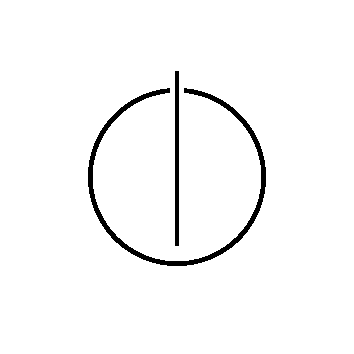
\includegraphics[width=4cm]{styles/informat.png}
  \end{figure}
  
  \end{center}
%	\clearemptydoublepage
%	
%	% The titlepage for the CAMP report document.
% Included by MAIN.TEX


%--------------------------------------------------
% The title page
%--------------------------------------------------

% correct BCOR - undo at the end !!!
\def\bcorcor{0.15cm}
\addtolength{\hoffset}{\bcorcor}

\thispagestyle{empty}

 \vspace{10mm}
\begin{center}
	       \oTUM{4cm}
	   
	   \vspace{5mm}     
	   \huge FAKULT{\"A}T F{\"U}R INFORMATIK\\ 
	   \vspace{0.5cm}
	 \large DER TECHNISCHEN UNIVERSIT{\"A}T M{\"U}NCHEN\\
        
	\end{center}
		

\vspace{5mm}
\begin{center}

   {\Large \doctype}

  \vspace{5mm}
  
  {\LARGE \title}\\
  
  
  \vspace{5mm}
  
  
  {\LARGE  \titleGer}\\
  
  
  \vspace{5mm}

    %\hfill
    \begin{tabular}{ll}
	   \Large Author:        & \Large \author \\[2mm]
	   \Large Supervisor:    & \Large Prof. Dr. Claudia Eckert \\[2mm]				
	   \Large Advisor:	 & \Large M.Sc. Paul Muntean \\[2mm]
	   \Large Date:          & \Large November 7th, 2016
	 \end{tabular}
	 
	 
	 \begin{figure}[h!]
  \centering
   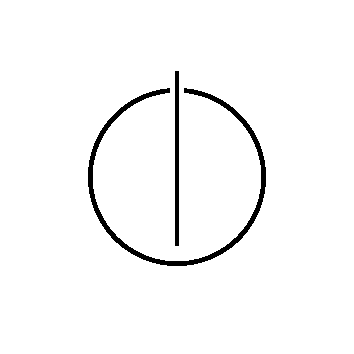
\includegraphics[width=4cm]{styles/informat.png}
  \end{figure}
   

\end{center}

% undo BCOR correction
\addtolength{\hoffset}{\bcorcor}
	
	
%	\input{components/cover_maschmeyer}
	\clearemptydoublepage
	
	% The titlepage for the CAMP report document.
% Included by MAIN.TEX


%--------------------------------------------------
% The title page
%--------------------------------------------------

% correct BCOR - undo at the end !!!
\def\bcorcor{0.15cm}
\addtolength{\hoffset}{\bcorcor}

\thispagestyle{empty}

 \vspace{10mm}
\begin{center}
	       \oTUM{4cm}
	   
	   \vspace{5mm}     
	   \huge FAKULT{\"A}T F{\"U}R INFORMATIK\\ 
	   \vspace{0.5cm}
	 \large DER TECHNISCHEN UNIVERSIT{\"A}T M{\"U}NCHEN\\
        
	\end{center}
		

\vspace{5mm}
\begin{center}

   {\Large \doctype}

  \vspace{5mm}
  
  {\LARGE \title}\\
  
  
  \vspace{5mm}
  
  
  {\LARGE  \titleGer}\\
  
  
  \vspace{5mm}

    %\hfill
    \begin{tabular}{ll}
	   \Large Author:        & \Large \author \\[2mm]
	   \Large Supervisor:    & \Large Prof. Dr. Claudia Eckert \\[2mm]				
	   \Large Advisor:	 & \Large M.Sc. Paul Muntean \\[2mm]
	   \Large Date:          & \Large November 7th, 2016
	 \end{tabular}
	 
	 
	 \begin{figure}[h!]
  \centering
   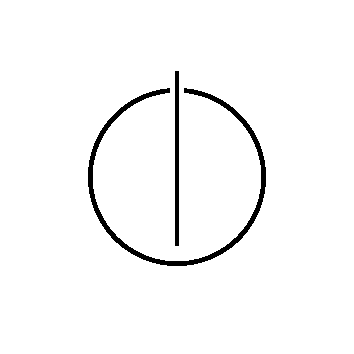
\includegraphics[width=4cm]{styles/informat.png}
  \end{figure}
   

\end{center}

% undo BCOR correction
\addtolength{\hoffset}{\bcorcor}
	
	
	\clearemptydoublepage


\thispagestyle{empty}
\selectlanguage{german}
	\vspace*{0.8\textheight}
	\noindent
	I confirm that this master’s thesis in informatics is my own work and I have documented
        all sources and material used.
	
	\vspace{15mm}
	\noindent
	M{\"u}nchen, den \today \hspace{5cm} \author
\selectlanguage{english}
\newpage
	
	\clearemptydoublepage
\phantomsection
\addcontentsline{toc}{chapter}{Acknowledgements}	


%\chapter*{Acknowledgements}

\vspace*{2cm}

\begin{center}
{\Large \bf Acknowledgments}
\end{center}

\vspace{1cm}




If someone contributed to the thesis... might be good to thank them here.
	
	
%MA Thesis
% Applications like firefox, chrome, mysql, postgresql or nginx are written in C/C++ 
% mostly for performance reasons or to have better control thereover, availability 
% and a vast number of third party libraries are other strong reasons. Yet using 
% these languages comes at the price of allowing code reusage attacks, as up to this
% day buffer overflows and other memory corruption exploits are haunting the various
% projects using C/C++. This is not the main focus, but only a prerequisite of the 
% attacks we are going to discuss. The language c++, which initially was built based
% on C introduced the concept of inheritance to allow for more flexible designs. 
% This modelled by storing a pointer to a table that stores the virtual functions 
% of the particular object. The relatively recently discovered COOP exploits and its
% successors leverage this pointer to change the control flow hijacking the attacked
% program. Although C does not employ the concept of virtual calls, it is still 
% attackable by modifying global code pointers as shown in the Control Flow Bending
% paper.
% 
% While there exists extensive work to protect binaries from the source level, 
% one might not have access to the the sourcecode or compilation process, 
% therefore binary based solutions must also be considered , of which there
% are near to none that can mitigate COOP exploits. In this thesis, we present
% \textsc{TypeShield} a tool implemented ontop of the principles introduced by
% TypeArmor, which reportedly can mitiagte COOP attacks to a certain extent. 
% We partially verify the results of TypeArmor and implement our own matching
% schema based on the parameter wideness of callsites and calltargets. 
% Our classification schema achieves an additional reduction of the possible
% calltargets per callsite of up to 20\% with an overall reduction of about 
% 9\% when comparing to parameter count based aproaches.



%Paper abstract
High security, high performance and high availability 
applications such as the Firefox and Chrome web browsers 
are implemented in C/C++ for modularity, performance and 
compatibility to name just a few reasons.
Virtual functions, which facilitate late binding,
are a key ingredient in facilitating run-time polymorphism
in C++ because it allows and object to use general (its own) 
or specific functions (inherited) contained in the class hierarchy.
However, because of the specific implementation of late binding,
which performs no verification in order to check where an indirect call site 
(virtual object dispatch through virtual pointers (\textit{vptrs})) is allow to
call inside the class hierarchy, this opens a large attack surface which
was successfully exploited by the COOP attack.
Since manipulation (changing or inserting new \textit{vptrs}) violates the 
programmer initial pointer semantics and allows an attacker to
redirect the control flow of the program as he desires, \textit{vptrs} corruption
has serious security consequences similar to those of other 
data-only corruption vulnerabilities.
Despite the alarmingly high number of \textit{vptr} corruption
vulnerabilities, the \textit{vptr} corruption problem has not
been sufficiently addressed by the researchers.

In this paper, we present \textit{TypeShild}, a run-time \textit{vptr} corruption
detection tool. It is based on executable instrumentation at load time
and uses a novel run-time type and function parameter counter technique
in order to overcome the limitations of current approaches and efficiently
verify dynamic dispatching during run-time.
In particular, \textit{TypeShild} can be automatically and easily used
in conjunction with legacy applications or where source code is missing.
It achieves higher caller/caller matching (precision) and with reasonable
run-time overhead.
We have applied \textit{TypeShild} to real life software such as
web servers, JavaScript engines, FTP servers and large-scale software
including Chrome and Firefox browsers, and were able to efficiently
and with low performance overhead to protect this applications from 
\textit{vptr} corruptions vulnerabilities.
Our evaluation shows that our target reduction schema achieves an additional
reduction of the possible call targets per call-site of up to 
20\% with an overall reduction of about 9\% when comparing to other
parameter count based approaches.


	\tableofcontents
  
  \clearemptydoublepage

\phantomsection
\addcontentsline{toc}{chapter}{Outline of the Thesis}

\begin{center}
	\huge{Outline of the Thesis}
\end{center}




%--------------------------------------------------------------------
\section*{Part I: Introduction and Theory}

\noindent {\scshape Chapter 1: Introduction}  \vspace{1mm}

\noindent  This chapter presents an overview of the thesis and it purpose. Furthermore, it will discuss the sense of life in a very general approach.  \\

\noindent {\scshape Chapter 2: Theory}  \vspace{1mm}

\noindent  No thesis without theory.   \\

%--------------------------------------------------------------------
\section*{Part II: The Real Work}

\noindent {\scshape Chapter 3: Overview}  \vspace{1mm}

\noindent  This chapter presents the requirements for the process.

	\mainmatter
	
	
		% ---------------------------------------------------------------------------
		%
		%Introduction and Background Theory
		%
		% ---------------------------------------------------------------------------
		\part[Introduction and Theory]{Introduction and Theory}
		\label{part:introAndBackgroundTheory}
		\section{Introduction}
\label{chapter:Introduction}
In this Chapter we present the motivation of our work in Section~\ref{Motivation}.
Section~\ref{Contribution} presents the contribution of our work.
Finally, Section~\ref{Outline} depicts the thesis outline.

\textbf{Motivation.}
\label{Motivation}
Control-Flow Integrity (CFI)~\cite{abadi:cfi2, abadi:cfi} is one of the most used techniques to secure program execution flows against advanced Code-Reuse Attacks (CRAs).
Advanced CRAs such as the recently published COOP~\cite{schuster:coop} and its extensions \cite{crane:readactor++} or the attacks described by the Control Flow Bending paper \cite{carlini:bending} are able to bypass most traditional CFI solutions, as they focus on indirect callsites, which are not as easy to decide at compile time.

This is a problem for applications written in C++, as one of its principle is inheritance and virtual functions. The concept of virtual functions allows the programmer to overwrite a virtual function of the baseclass with his own implementation. While this allows for much more flexible code, this flexibility is the reason COOP actually works. The problem is that in order to implement virtual functions, the compiler needs to generate a table of all virtual functions for each class containing them and provide each instanciation of such a class with a pointer to said table. COOP now leverages a memory corruption to inject their own object with a fake virtual pointer, which basically gives him control over the whole program, while the control flow still looks genuine, as no code was replaced. 

There exist several source code based solutions that either insert runtime checks during the compilation of the program like SafeDispatch \cite{safedispatch:jang}, ShrinkWrap \cite{haller:shrinkwrap} or IFCC/VTV \cite{vtv:tice}, which is the solution it is based on. Others modify and reorder the contents of the virtual table as their main aspect like the paper by Bounov et al \cite{bounov:interleaving}. While the recently published redactor++ \cite{crane:readactor++} implements a combination of those ideas.

While this might seem that only C++ is vulnerable, while C is safe, this notion is wrong, as the Control Flow Bending paper \cite{carlini:bending} proposes attacks on nginx leveraging global function pointers, which are used to provide configurable behaviour.

As previously mentioned, there exist many solutions when one tries to tackle this problem while access to the application in question is provided. However, when we are faced with proprietary third party binaries, which are provided as is and without the actual sourcecode, the number of tools that can protect against COOP or similar attacks is rather low.

TypeArmor~\cite{veen:typearmor} is such a tool that implements a fine grained forward edge CFI solution for binaries. It calculates invariants for calltargets and indirect callsites based on the number of parameters they use by leveraging static analysis of the binary, which then is patched to enforce those invariants during runtime. However, as of today we are not able to access the source code of TypeArmor, which is why we implement our own approximation of the tool.

The main shortcoming of TypeArmor is that even with high precision in the classification of calltargets and callsites, one cannot exclude calltargets with lower parameter number from callsites, for one due compatability and also due to variadic functions, which are a special case in themselves. This basically means that when a callsite prepares 6 parameters, it is able to call all address taken functions.


We implemented \textit{TypeShield} to show a possible remedy of this problem by introducing parameter types into the classification of callsites and calltargets. 

\textbf{Contribution.}
\label{Contribution}
The goals of our thesis are twofold. First we attempt to verify the results as provided by the TypeArmor paper. Second, implement our own classification schema to fix some of the shortcomings of previous binary based approaches to further mitigate advanced code reuse attacks.

Our main contribution is thus the design and implementation of callsite and calltarget classification schema that is based on the wideness of parameters alone. We implemented configurable reaching and liveness analysis algorithms that operate on the full set of general purpose integer registers of a x86-64 CPU and evaluated various path merge operators. Although the basic idea of our aproach to rely only on the wideness of a type is rather simple, we still achieved a reduction of up to 20\% less callsites per calltarget with an overall of about 9\% when compared to our implementation of a parameter count based matching schema.


Furthermore, we implemented an approximation of the matching schema employed by TypeArmor proposed by \cite{veen:typearmor}, because we had no access to their sourcecode and could achieve similar results regarding parameter matching, partially verifying their results.

\textbf{Outline.}
\label{Outline}
The remainder of this thesis is organized as follows.
Chapter~\ref{chapter:TypeShild Overview} contains a high level overview of \textit{TypeShield}.
Chapter~\ref{chapter:Design} describes the theory used and decisions made during the design of \textit{TypeShield}.
Chapter~\ref{chapter:Implementation} briefly presents the implementation details of our tool.
Our \textit{TypeShield} implementation is evaluated and discussed in
Chapter~\ref{chapter:Evaluation} and Chapter~\ref{chapter:Discussion}, respectively.
Chapter~\ref{chapter:Related_Work} surveys related work.
Finally, Chapter~\ref{chapter:Future_Work} highlights several future venues of research while
Chapter~\ref{chapter:Conclusion} concludes this thesis.



		
		
		%
		%% ---------------------------------------------------------------------------
		%%
		%% Fully Automated Calibration for Ultrasound
		%%
		%%% ---------------------------------------------------------------------------
		\part[The 2nd Part]{The Second Part}
		\label{part:secondP}
		
		
		% ---------------------------------------------------------------------------
		%
		% Appendix
		%
		% ---------------------------------------------------------------------------
		
		\part*{Appendix}
		\addcontentsline{toc}{part}{Appendix}
		
		\appendix %---------------------------------------
		
		\chapter{Detailed Descriptions}
%\section{Detailed Validation Results}
\label{chapter:DetailedDescriptions}
Here come the details that are not supposed to be in the regular text.
		
	


  \clearemptydoublepage
  
	\bibliography{bibliography/literature}
	
 
\end{document}

